

\subsubsection{Dynamixel Servo PID}
In each Dynamixel servo there is an build in controller. The controller contain a feedback loop with an implemented PID controller with limiters to ensure that servos rotation-velocity do not exceed a lower and a higher threshold\cite{PIDmxx}. The feedback loop and the PID controller can be customised to fit the purpose of a given task.
\begin{figure}[H]
    \centering
    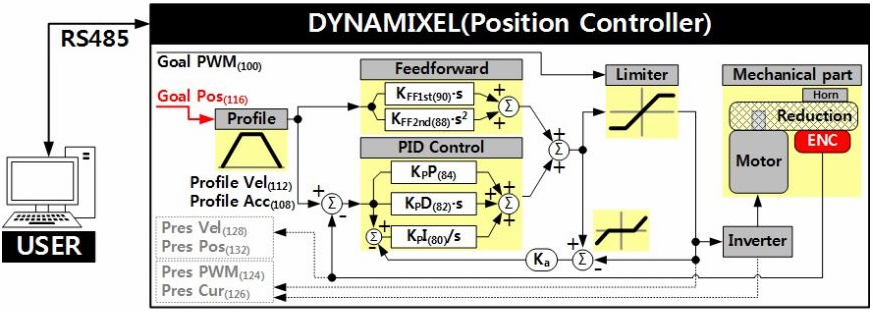
\includegraphics[width=\textwidth]{Figures/Technical_figures/PIDMX.PNG}
    \caption{Internal PID controller in the Dynamixel servos\cite{PIDmxx}}
    \label{fig:PIDMX}
\end{figure}

The servos positioning and velocity is analysed through the use of an encoder, placed on the gearing of the motor.  